\chapter{Background and Prior Work}\label{ch:background}
% Background intro. Explaining what you've included in this section. 
% TODO: update if you add more to background
\todo{In this chapter}, we begin by discussing the problem of network side-channel attacks and exploring various proposed mitigations for such attacks. 
Following that, we present a comprehensive definition of differential privacy (DP), outline its key properties, and highlight its primary applications, thereby setting the foundation for elucidating our differentially private traffic shaping mechanism. 

\section{QUIC Transport Protocol}

QUIC is a modern transport layer protocol specifically developed to enhance the performance of HTTPS traffic~\cite{langley2017quic}.
In the traditional IP stack model, QUIC encompasses both the Transport layer and the Application layer.
In other words, QUIC is a user-space transport layer protocol built on top of UDP. 
Using UDP packets as the transport layer carrier allows QUIC packets to traverse current network infrastructure developed for TCP/UDP protocols such as middleboxes.
On the top of UDP, QUIC provides transport functionalities of flow control, loss recovery, encryption, and congestion control.
Unlike TCP, QUIC mitigates head-of-the-line blocking delays by introducing a novel data structuring abstraction known as streams. 
QUIC is now standardized under RFC 9000~\cite{rfc9000}, and the details of design and implementation of the protocol is well beyond the scope of this thesis.
We, however, provide a brief overview of QUIC features and functionalities that are relevant to the design of {\sys}.




\subsection{QUIC Connections}
A QUIC connection is a shared state between a client and a server.
At the initiation of each connection, a handshake phase takes place where the two endpoints engage in a cryptographic handshake protocol~\cite{rfc9001} to establish a shared secret and negotiate the application protocol.
This handshake process ensures mutual consent for communication and establishes connection parameters.

Each connection has two unique IDs, source connection ID, and destination connection ID.
By assigning each connection unique identifiers (ID), the potential changes in addressing layers at lower network levels, such as UDP and IP, do not result in incorrect packet delivery at the receiving endpoint.
Furthermore, routers can leverage existence of destination connection ID to route QUIC packets in the network to the correct endpoint.
During the handshake, one endpoint establishes the Source Connection ID by setting it in the packet header.
Similarly, the other endpoint determines the Destination Connection ID.

QUIC provides three ways to terminate a connection: idle timeout, immediate close, and stateless reset.
Each endpoint can specify an idle timeout in its transport parameters.
If the idle timeout duration elapses without any data exchange between the endpoints, the endpoint will silently close the connection (\ie without explicitly notifying the other endpoint). 
The other connection termination method is the immediate close. 
To promptly terminate the connection, an endpoint transmits \texttt{CONNECTION\_CLOSE} frame. 
This frame triggers the immediate termination of all streams within the connection.
Upon sending a \texttt{CONNECTION\_CLOSE} frame, the sender promptly terminates the connection without waiting for acknowledgment from the receiver.
A stateless reset is available as a fallback choice for an endpoint that lacks access to the connection state.
In cases of a crash or outage, it is possible for endpoints to continue sending data to an endpoint that cannot properly maintain the connection.
In such cases, the endpoint without the connection state issues the stateless reset, terminating the connection and its state machine locally.




\subsection{QUIC Streams}
QUIC's streams offer a lightweight and ordered way for applications to send byte-streams.
These streams can be either unidirectional or bidirectional, depending on the specific needs of the application.
Within a connection, each stream is identified with a new ID.
A stream ID is 62 bit integer.
Either of endpoints can create a stream just by sending data with a new stream ID. 
There are no restrictions on the number of simultaneous streams (other than, of course, the maximum number of unique IDs) or the length of each individual stream.
QUIC assigns different priorities to different streams based on the applications' requirement.
The prioritization of streams within a connection can have a substantial impact on the performance of applications.
Each stream has a dedicated header with 5 major fields: Type, Stream ID, Offset, and Data Length.
The stream header within a packet is encrypted, ensuring that adversaries are unable to discover the active streams in a connection.
Either of endpoints can terminate streams by sending a \texttt{STREAM\_RESET} frame to the other one.
In a bidirectional stream, both endpoints should send \texttt{STREAM\_RESET} message to completely terminate a stream.

% \subsection{QUIC Congestion and Flow Control}
% \subsubsection{Flow Control}
% To prevent a fast or malicious sender from overwhelming receivers' buffer, receivers must proactively limit the amount of data a sender can send.
% QUIC can perform flow control at two levels: The receiver controls the maximum amount of data the sender can send on a per-stream basis, as well as across all streams within a connection. 
% The receiver sets the initial limits for stream and connection flow controls during the handshake. 
% During the handshake, the receiver establishes the initial limits for both stream and connection flow controls. Throughout the connection, if the receiver needs to adjust the limits for a specific stream, it sends \texttt{MAX\_STREAM\_DATA} frames to the sender.
% Similarly, to change the limit for overall connection, the receiver sends \texttt{MAX\_DATA} frames to the sender.

% \subsubsection{Congestion Control}
% QUIC does not standardize any specific method of congestion control.
% Instead, it provides the necessary feedback mechanism to implement congestion control.
% The modular design of congestion control makes QUIC more flexible, allowing applications to implement a congestion mechanism that aligns with their specific requirements.
% As the default congestion control mechanism, however, QUIC uses a sender specified congestion controller similar to TCP NewReno~\cite{rfc6582}.
% Given the limitations of this thesis, a comprehensive explanation of TCP NewReno is outside its scope.
% For a more in-depth understanding of this mechanism, we kindly refer readers to the RFC, which provides detailed information and insights.


\section{Differential Privacy}\label{sec:dp-background}
% Subsection intro. Elaborate on origins of DP. Why it is useful.
Data scientists always strive to understand the general properties of a population. 
To answer questions concerning the etiology of a disease, factors contributing to a societal phenomenon, or the consequences of an economic policy, researchers collect data from individual people. They then process this data to calculate population-level statistics and propose solutions based on these aggregated statistics.
Ensuring the privacy of individuals who have contributed to these studies is of utmost importance from both ethical and legal perspectives.
In fact, the intended goal of all scientific studies is to collect valuable information about the targeted population not individual people within the population. 
However, it is impossible to learn useful information about a population while learning \textit{nothing} about individuals, leading to a paradox between usefulness of a dataset (\ie utility) and its privacy. 
Differential Privacy (DP) addresses this paradox by quantifying the extent of privacy leakage for individuals in a dataset when publishing its statistics.
Within the framework of Differential Privacy (DP), the aforementioned paradox transforms into an adjustable trade-off between the utility of data and the preservation of privacy. 

In the rest of this section, we provide the formal definition of differential privacy, highlight its main properties, and explore its potential application in the domain of traffic shaping.


%
%% 
%% Definition
%%
%


\subsection{Definitions}\label{subsec:background-dp-definitions}
A database $D$ has a fixed number of entries, where each individual data point is stored in one entry.
Following the notation proposed by Dwork \etal \cite{dwork2014algorithmic}, we represent databases by their histograms: $D \in \dbSpace$. 
In this representation, every entry $D_i$ of the database $D$ represents the number elements of type $i \in \mathcal{X}$.
\\  
Within the DP context, we define a \textit{query} as a function that operates on a database. 
Any computation performed on a database, regardless of its codomain, can be regarded as a query executed on that database.
The primary objective of differential privacy is to offer meaningful population-level information for queries executed on a database, all while protecting the privacy of individual data points within the database.
Intuitively, small changes in a database should not significantly impact the outcome of a query.
To further clarify the terms "small changes" and "significant impact", we provide definitions for neighboring databases and query function sensitivity, respectively.
\\
We measure the difference between two databases with a distance metric $\rho(D, D')$.
\begin{definition}[Neighboring databases]
  Given a distance metric $\rho$, we refer to two databases $D, D' \in \dbSpace$ as neighboring databases, if and only if $\rho(D, D') \leq 1$.             
\end{definition}
\noindent In the standard DP definition, the distance metric is simply the number of different data entries in two databases (\ie Hamming distance).
However, Chatzikokolakis \etal \cite{chatzikokolakis2013broadening} show that DP applies to a general definition of distance metrics.
\\
To quantify the extent to which a single data point can influence the outcome of a query in worst-case, we introduce the concept of sensitivity. 
\begin{definition}[$l_p$-Sensitivity]
  \label{def:norm-sensitivity}
  The $l_p$-sensitivity of a query function $f$ is:
  \begin{equation*}
    \Delta_p f = \max_{D, D'} \|f(D) - f(D')\|_p 
  \end{equation*}
where $\rho(D, D') \leq 1$ (\ie $D$ and $D'$ are neighboring databases).
\end{definition}
\noindent
Differential Privacy involves randomization of query outputs. We define a randomized algorithm as follows.
\begin{definition}[Randomized algorithm]
  \label{def:randomized-algorithm}
  A randomized algorithm $M$ with the domain $A$ and discrete range $B$, for any given $a \in A$ and $b \in B$ outputs $M(a)= b$ with probability of $(M(a))_b$.
\end{definition}

With all the necessary components in place, we are now prepared to present the formal definition of differential privacy.
\begin{definition}[Differential privacy]
  \label{def:dp}
  A randomized algorithm $M: \dbSpace \rightarrow \mathbb{R}$ is $(\varepsilon, \delta)$-differentially private if for all ${S} \subseteq Range(M)$ and for  all $D, D' \in \dbSpace$ such that $\rho(D, D') \leq 1$, we have:
  \begin{equation*}
    \Pr[M(D) \in S] \leq \exp(\varepsilon)\Pr[M(D') \in S] + \delta
  \end{equation*}
\end{definition}
\noindent
Indeed, Differential Privacy (DP) is a definition rather than a specific algorithm.
It provides a framework for ensuring privacy guarantees in various randomized algorithms. Multiple randomized algorithms can achieve $(\varepsilon, \delta)$-privacy for a given set of databases, each with different characteristics. 
Intuitively, given an output, with probability $1-\delta$ the log likelihood ratio of running the algorithm $M$ on databases $D$ and $D'$ is bounded by $\varepsilon$.
This bound ensures that the presence or absence of any individual's data in the database has a limited impact on the likelihood of obtaining a particular output.
The smaller $\varepsilon$ implies that both neighboring databases are equally likely to generate the output, resulting in more privacy.
The parameter $\varepsilon$ is commonly referred to as \textit{privacy loss} within the context of DP.
The parameter $\delta$ determines the failure probability of a differential private mechanism and is typically expected to have a small value (\ie smaller than $10^{-5}$).


%
%% 
%% Properties
%%
%

\subsection{Properties}\label{subsec:background-dp-properties}
In this section, we explore the key properties of Differential Privacy as a privacy framework.


% ROBUSTNESS TO AUXILIARY INFORMATION.
\subsubsection{Robustness to auxiliary information}
\label{subsubsec:dp-auxiliary}
The definition of Differential Privacy does not make any assumptions regarding the prior knowledge of the adversary. 
In other words, regardless of the adversary's prior knowledge, the information gained by the adversary after observing the output of a differentially private algorithm $M$ remains within the bounds specified by Differential Privacy. 
\begin{proposition}
  \label{prop:auxiliary}
  Assume that the adversary has a prior $\Pr(D)$ over the set of all possible databases $D, D' \in \dbSpace$, given the output $S$ of a $(\varepsilon, \delta)$-DP algorithm $M: \dbSpace \rightarrow \mathbb{R}$, for all $D, D' \in \dbSpace$ such that $\rho(D, D') \leq 1$, we have: 
  \begin{equation*}
    \frac{\Pr(D|S)}{\Pr(D'|S)} \leq \exp(\varepsilon) \frac{\Pr(D)}{\Pr(D')}
  \end{equation*}
\end{proposition}
In broad terms, robustness to auxiliary information in the context of Differential Privacy is similar to the security semantics of cryptographic algorithms. 
For instance, consider a scenario where an adversary possesses the knowledge that the content of an encrypted message is either a picture of a car or a picture of a tree.
In this case, observing the encrypted message does not provide any additional evidence to indicate which of the two possibilities is more likely to be the true message.
In DP, nevertheless, observing the results of private queries does change the prior knowledge of the adversary.
However, this change remains within the boundaries defined by DP and does not exceed them.

% POST-PROCESSING
\subsubsection{Post-processing}
\label{subsubsec:background-dp-postprocessing}
Differential Privacy guarantees are resilient to post-processing of the output from a DP algorithm.
In fact, in the absence of any additional knowledge, the adversary is unable to undermine the guarantees of Differential Privacy simply by processing the output of the algorithm.
\begin{proposition}
  \label{prop:post-processing}
  Consider $M: \dbSpace \rightarrow R$ as a $(\varepsilon, \delta)$-differentially private algorithm, and let $g: \mathbb{R} \rightarrow \mathbb{R}$ be an arbitrary randomized mapping, then $g(M(.)): \dbSpace \rightarrow \mathbb{R}$ is $(\varepsilon, \delta)$-differentially private. 
\end{proposition}
\noindent
This implies that regardless of the complexity of a procedure, as long as the inputs are differentially private, the output is guaranteed to maintain the same level privacy.
The post-processing property of Differential Privacy can be especially advantageous when dealing with systems that have information bottlenecks, such as situations where results from multiple calculations are aggregated at a single stage.
In such systems, by applying a differentially private algorithm to the information bottleneck, the guarantee of Differential Privacy extends to the output of the entire system. 
We specifically utilize post-processing property of Differential Privacy in the design of both the {\sys} shaping mechanism and the {\sys} middlebox. 

% PRESERVATION UNDER ADAPTIVE SEQUENTIAL COMPOSITION.
\subsubsection{Self-Composition}\label{subsubsec:background-dp-composition}
The simultaneous release of results from multiple differentially private algorithms maintains the differential privacy guarantee.
This property facilitates the modular construction of differentially private algorithms, allowing multiple DP algorithms to be combined to create more sophisticated and advanced algorithms.
Furthermore, the composition theorem enables us to compute the privacy parameters associated with the sequential release of a differentially private algorithm output, thereby facilitating multiple releases of the same DP output.
There are multiple variants of composition theorem, and we with the simplest form of composition.
\begin{proposition}[Basic composition theorem]
\label{prop:basic-composition}
  Let $M_i: \dbSpace \rightarrow \mathbb{R}$ be an $(\varepsilon_i, \delta)$-differentially private algorithm for $i \in [k]$. Then, the combination of these $k$ algorithms, $M_{[k]}: \dbSpace \rightarrow \Pi_{i=1}^{k}\mathbb{R}$ is $(\sum_{i=1}^{k}\varepsilon_i, \sum_{i=1}^{k}\delta_i)$-differentially private.  
\end{proposition}
Basic composition theorem states that the privacy loss resulting from the combination of multiple differentially private algorithms is equal to the aggregate of their individual privacy losses.
While functional, the basic composition theorem tends to overestimate the privacy loss of combined DP algorithms.
The advanced composition theorem offers a more precise and rigorous bound for the aggregated privacy loss incurred by multiple differentially private algorithms. 
\begin{proposition}[Advanced composition theorem]
\label{prop:advanced-composition}
  Let $M_i: \dbSpace \rightarrow \mathbb{R}$ be an $(\varepsilon, \delta)$-differentially private algorithm for $i \in [k]$. Then, the combination of these $k$ algorithms, $M_{[k]}: \dbSpace \rightarrow \Pi_{i=1}^{k}\mathbb{R}$ is $(\varepsilon', k\delta+\delta')$-differentially such that:
  \begin{equation*}
    \forall \delta' \geq 0: \varepsilon' = \sqrt{2k\ln(1/\delta')}\varepsilon + k\varepsilon(e^{\varepsilon} - 1)
  \end{equation*}
\end{proposition}
It is important to note that this form of composition theorem is only applicable to differentially private algorithms that share the same privacy parameters.
More sophisticated versions of the composition theorem exist, offering tighter privacy bounds~\cite{kairouz2015composition, mironov2017renyi}.
We particularly use R{\'e}nyi Differential privacy to calculate the privacy loss of our differentially private shaping mechanism.

\subsection{Mechanisms}\label{subsec:background-dp-mechanism}
\Cref{def:randomized-algorithm} provides a general definition of a randomized algorithm, while \Cref{def:dp} outlines the specific criteria that a randomized algorithm must satisfy to be considered differentially private (\ie DP mechanism).
In this section, we will explore the two most commonly used differentially private mechanisms: the Laplace mechanism and the Gaussian mechanism\cite{dwork2014algorithmic}.
\begin{definition}[Laplace Mechanism]\label{def:laplace-mechanism}
  Given any function $f: \dbSpace \rightarrow \mathbb{R}^k$ the Laplace mechanism is defined as:
  \begin{equation*}
    \mathcal{M}(x, f, \varepsilon) = f(x) + (Y_1, Y_2, \dots, Y_k)
  \end{equation*}
  where $Y_i$ are i.i.d random variables from Laplace distribution with probability density function of $Lap(\Delta_1 f/\varepsilon)$, and $\Delta_1 f$ is $l_1$-sensitivity of function $f$ (see \Cref{def:norm-sensitivity}).
\end{definition}
The Laplace mechanism is relatively easy and straightforward. 
Intuitively, it just adds a random variable driven from a Laplace distribution to the result of the query.
The variance of this random variable quantifies the privacy of query results, as a higher variance makes it more challenging for adversaries to infer the true result of the query.
\begin{proposition}
  The Laplace mechanism of \Cref{def:laplace-mechanism} is $(\varepsilon, 0)$-differentially private. 
\end{proposition}
\noindent
We omit the proof here; you can refer to the work of Dwork\etalc{dwork2014algorithmic} for a detailed proof. 
As we can see in \Cref{def:laplace-mechanism}, the failure probability of Laplace mechanism, $\delta$, is 0.
In broad terms, a mechanism can compromise failure rate $\delta$ to add less noise to query results while achieving same values for privacy loss $\varepsilon$.
\begin{definition}[Gaussian Mechanism]\label{def:gaussian-mechanism}
  Given any function $f: \dbSpace \rightarrow \mathbb{R}^k$ the Gaussian mechanism is defined as:
  \begin{equation*}
    \mathcal{M}(x, f, \varepsilon, \delta) = f(x) + (Y_1, Y_2, \dots, Y_k)
  \end{equation*}
  where $Y_i$ are i.i.d random variables from Gaussian distribution $\mathcal{N}(0, \frac{2\Delta_2 f^2}{\varepsilon^2})\ln(\frac{1.25}{\delta})$, and $\Delta_2 f$ is $l_2$-sensitivity of function $f$ (see \Cref{def:norm-sensitivity}).
\end{definition}
We particularly design our differentially private traffic shaping mechanism using Gaussian mechanism at its core. 
We elaborate on this in \Cref{subsec:dp-shaping-mechanism}.

\subsection{R\'enyi Differential Privacy}
Despite widespread usage, straightforward interpretability,, and numerous applications of standard definition of $(\varepsilon, \delta)$-differential privacy, this concept does exhibit two primary limitations. 
First, the presence of the failure probability $\delta$ in this definition contradicts the guarantee of  plausible deniability associated with differential privacy since with probability $\delta$ the secret can be completely exposed.    
Secondly, as we mentioned in \Cref{subsec:background-dp-properties}, the desirable results of strong composition theorem only holds for homogeneous DP mechanisms.
In fact, Vadhan~\etalc{murtagh2015complexity} demonstrate that the generalization of advanced composition theorem to heterogeneous DP mechanisms (\ie $(\varepsilon_i, \delta_i)$-DP for different values of $\varepsilon_i$ and $\delta_i$) is P-hard.
To address these limitations, Mironov~\etalc{mironov2017renyi} propose a new definition of differential privacy based on the R\'enyi divergence~\cite{renyi1961measures}.
R\'enyi differential privacy (RDP) is strictly stronger than $\varepsilon, \delta$-DP, meaning that any $\varepsilon, \delta$-DP mechanism is RDP though the reverse does not hold true.
In this section, we explain the core concepts of R\'enyi differential privacy (RDP), elaborate on its properties, and highlight its connection to standard definition of DP.

\begin{definition}[R\'enyi divergence]
  for two probability distributions $P$ and $Q$, the R\'enyi divergence of order $\alpha > 1$ is defined as:
  \begin{equation*}
    D_{\alpha}(P||Q) \triangleq \frac{1}{\alpha-1} \log E_{x \sim Q}\left ( \frac{P(x)}{Q(x)} \right )
  \end{equation*}
\end{definition}
R\'enyi divergence simply measure the difference between two distributions $P$ and $Q$.
For $\alpha = \infty$, the R\'enyi divergence specifically defined as:
\begin{equation*}
  D_{\infty}(P||Q) \triangleq  \sup_{x \sim Q} \; \log \left ( \frac{P(x)}{Q(x)} \right ) 
\end{equation*}
We can see that the R\'enyi divergence with $\alpha=\infty$ is closely connected to $(\varepsilon, 0)$-DP definition.
\begin{proposition}
  A randomized algorithm $M: \dbSpace \rightarrow \mathbb{R}$ is $(\varepsilon, 0)$-differentially private iff for all $D, D' \in \dbSpace$ such that $\rho(D, D') \leq 1$, we have:
  \begin{equation*}
    D_{\infty}(P||Q) \leq \varepsilon
  \end{equation*} 
\end{proposition}
\noindent Next, we provide the formal definition of R\'enyi DP.
\begin{definition}[$(\alpha, \varepsilon)$-RDP]
  A randomized algorithm $M: \dbSpace \rightarrow \mathbb{R}$ is $(\alpha, \varepsilon)$-RDP if for all $D, D' \in \dbSpace$ such that $\rho(D, D') \leq 1$, we have:
  \begin{equation*}
    D_{\alpha}(\mathcal{M}(D)||\mathcal{M}(D')) \leq \varepsilon
  \end{equation*}
\end{definition}
\noindent Indeed, all the favorable attributes of the standard definition of differential privacy, including post-processing, self-composition, and robustness to auxiliary information, remain applicable to R\'enyi differential  privacy.
Particularly, the composition theorem has a simple representation in RDP.
\begin{proposition}[R\'enyi Composition]\label{prop:rdp-composition}
  Let $M_i: \dbSpace \rightarrow \mathbb{R}$ be an $(\alpha, \varepsilon_i)$-RDP algorithm for $i \in [k]$. Then, the combination of these $k$ algorithms, $M_{[k]}: \dbSpace \rightarrow \Pi_{i=1}^{k}\mathbb{R}$ is $(\alpha, \sum_{i=1}^{k}\varepsilon_i)$-RDP.   
\end{proposition}
\noindent For an in-depth proof, we direct readers to the R\'enyi differential privacy paper~\cite{mironov2017renyi}.
So far, we explained three methods to calculate the aggregated privacy loss of multiple releases of differentially-private mechanism.
These methods are basic composition theorem, advanced combination theorem, and R\'enyi composition theorem.
The goal of these methods is to provide a tight, accurate bound on aggregated privacy loss without overestimation. 
In simpler terms, a composition theorem is superior to another, if it can provably show that the aggregated privacy loss of a differentially-private mechanism, after multiple release of results, is smaller than the aggregated privacy loss indicated by the other mechanism.
A natural question is: \textit{What is the difference between all these mechanisms?}
To answer these questions, we calculate the privacy loss reported by these mechanisms for different number of queries (\ie varying number of differentially-private releases of results).
We fix epsilon and delta per query $0.2$ and $0.0001$ respectively, and report the final privacy loss for a given number of queries.
\begin{figure}[t]
  \centering
  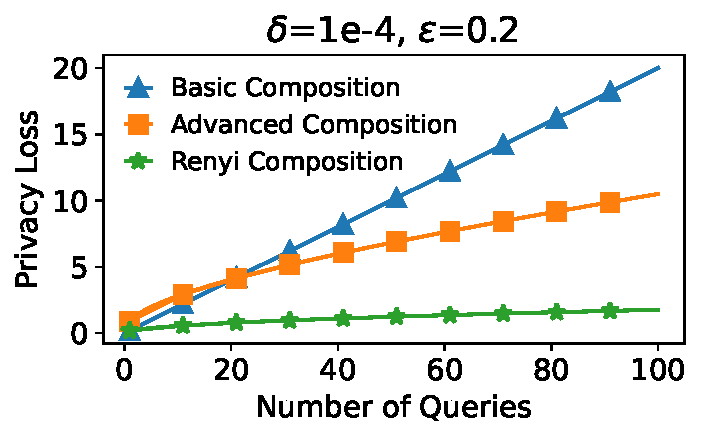
\includegraphics[width=\columnwidth]{plots/composition_comparison.pdf}
  \caption{Aggregated privacy loss of multiple queries reported by different composition methods}
  \label{fig:composition-comparison}
\end{figure}

\Cref{fig:composition-comparison} compares different methods for composing privacy loss of DP mechanisms.
We can see the effectiveness of R\'enyi methods as compared to others across all values for number of queries.
Advanced composition theorem also outperforms basic composition theorem for larger number of queries. 


As we mentioned earlier, $(\alpha, \varepsilon)$-RDP is strictly stronger than $\varepsilon, \delta$-DP. 
Next proposition shows how RDP implies standard DP.
\begin{proposition}\label{prop:rdp-better-than-dp}
  If $M: \dbSpace \rightarrow \mathbb{R}$ is an $(\alpha, \varepsilon)$-RDP mechanism, it is also $(\varepsilon + \frac{\log 1/\delta}{\alpha-1}, \delta)$-DP for any $0 < \delta < 1$. 
\end{proposition}
\noindent \Cref{prop:rdp-better-than-dp} enables us to interpret guarantees of R\'enyi differential privacy with semantics of standard differential privacy. 
Besides that, \Cref{prop:rdp-composition} provides us with the means to compose heterogeneous differentially private algorithms, while and at the end, with \Cref{prop:rdp-better-than-dp} we can still represent the final result using semantics of standard DP. 
In order to compute the privacy loss (\ie $\varepsilon$) of our differentially private shaping mechanism in \Cref{sec:dp-privacy-guarantees}, we use \Cref{prop:rdp-composition} referred to as $\textrm{DP\_compose}()$.

\section{Network Side Channel Defenses}\label{sec:ns-defenses}
% Section Intro, elaborate on the general theme of the section. 
In this section, we explore previous mitigation approaches proposed to address network side-channel attacks. 
We categorize these approaches into 4 general categories: 1- Static shaping methods, 2- Dynamic shaping methods, 3- Hybrid traffic shaping methods, 4- Adversarial traffic patterns. 




\subsection{Static Traffic Shaping}\label{subsec:static-traffic-shaping}
Static traffic shaping methods typically consist of two distinct phases: the profiling phase and the shaping phase.
During the profiling phase, the shaping mechanism collects user-specific information from the user's traffic traces.
This information can vary and may include details such as the exact traffic pattern, distribution of packet sizes, or timing of packet transmission.
The shaping mechanism then leverages this information during the shaping phase to transform users' traffic into a new pattern that ensures privacy with minimal overhead.
However, scaling static traffic shaping methods is challenging, or even impossible in many cases, due to the need for profiling numerous traffic traces.
% methods we are going to cover:
%% Walkie-Talkie 
%% Supersequence
%% Glove
%% Traffic morphing 
\subsubsection{Traffic Morphing}\label{subsubsec:traffic-morphing}
Traffic morphing~\cite{wright2009traffic} is a static approach for traffic shaping. 
In this method, the shaping mechanism alters the distribution of packet sizes in such a way that they resemble packets generated by a different website rather than the original website.
This helps to obfuscate the traffic and make it harder for eavesdroppers to associate the packets with their true source.
Traffic Morphing (TM) operates based on a technique known as \textit{Direct Target Sampling}.

First it collects the distribution of packets sizes for all websites in the dataset.
Then, Given a webpage $W$, TM randomly selects another webpage $W'$ from the dataset.
When selecting the target webpage $W'$, TM employs an optimization method to choose webpages that result in minimal overheads. 
Upon receiving each packet produced by $W$ with the size $l$, TM samples a packet size $l'$ from the distribution of $W'$. 
If $l' > l$, TM pads the outgoing packet with dummy data to match the size $l'$. 
On the other hand, if $l' < l$, TM sends $l'$ bytes and continues sampling from the distribution of $W'$ until all bytes of the original packet have been transmitted.
It is important to emphasize that the traffic morphing method does not hide the timing or duration of bursts of traffic.
Therefore, an adversary can still exploit these features of traffic traces to potentially reveal users' information based on their traffic patterns, even when traffic morphing is deployed~\cite{dyer2012peek}.


\subsubsection{Walkie-Talkie}\label{subsubsec:walkie-talkie}
Wang\etalc{wang2017walkie} propose \textit{Walkie-Talkie} as a new defense mechanism implemented in browsers to hide traffic shape of sensitive websites.
\textit{Walkie-Talkie} requires browsers modification to change the default full-duplex communication to half-duplex mode.
In full-duplex communication, multiple servers are actively transmitting web page data to the client, while the client concurrently submits additional resource requests, potentially to different servers.
In half duplex mode, on the other hand, the client only sends requests after the web servers have satisfied all previous requests.
Using half-duplex mode enables \textit{Walkie-Talkie} to change communication to a sequence of bursts of data between one client and one server at a time. 
\textit{Walkie-Talkie} represents each burst sequence $s$ as follows:
\begin{equation*}
  s = \{(b_{1+}, b_{1-}), (b_{2+}, b_{2-}), \dots \}
\end{equation*}
where $b_{i+}$ represents the size for the $i$th outgoing burst, and $b_{i-}$ represents the size for the $i$th incoming burst for sequence $s$.
\\
For any sensitive website $W$, \textit{Walkie-Talkie} first extract the burst sequence $s$.  
Then, using a similar approach to Traffic Morphing~\cite{wright2009traffic}, \textit{Walkie-Talkie} chooses a decoy website $W'$ with burst sequence of $s'$.
At the transmission time, \textit{Walkie-Talkie} reshapes the burst sequence of $s$ to sequence $\hat{s}$ such that:
\begin{equation*}
  (\hat{b}_{i+}, \hat{b}_{i-}) = (\max(b_{i+}, b_{i+}'), \max(b_{i-}, b_{i-}'))
\end{equation*}
where $\hat{b}_{i+}$, $b_{i+}$, and $b_{i+}'$ represent the size for the $i$th outgoing burst in sequences of shaped traffic $\hat{s}$, original webpage $s$, and decoy webpage $s'$ respectively.
The same notation used for incoming burst sizes.
Therefore, if an adversary observes the sequence $\hat{s}$, it can not ascertain whether the users accessed $W$ or $W'$.
Choosing multiple decoy burst sequences for any sensitive can further increase the privacy of \textit{Walkie-Talkie}.

Essentially, \textit{Walkie-Talkie} use as a clustering technique for shaping traffic, conceptually similar to Supersequence~\cite{wang2014supersequence}, Glove~\cite{nithyanand2014glove}, and Tamaraw~\cite{cai2014systematic}.
It maps the traffic shapes of various web pages to the same pattern, effectively rendering them indistinguishable for potential adversaries.
The advantages of the \textit{Walkie-Talkie} are: it adds small overheads compared to other defenses, requires minimal computation to extract the burst sequence of shaped traffic, and stores small metadata to for decoy webpages.
On the other hand, it had several disadvantages. 
First, \textit{Walkie-Talkie} requires browser modification.  
Secondly, similar to most of the static traffic shaping methods, \textit{Walkie-Talkie} should identify the burst sequence of a webpage before its transmission.
Finally, the adoption of half-duplex mode in browsers imposes a notable constraint on the scalability of this approach, as numerous applications, such as video streaming and file downloading, require multiple and simultaneous communications with web servers.


% ---------------------------------------------------% 
% ---------------------------------------------------% 
% ---------------------------------------------------% 
% ---------------------------------------------------% 
% ---------------------------------------------------% 

\subsection{Dynamic Traffic Shaping}\label{subsec:dynamic-traffic-shaping}
In these methods, the traffic shaping defense mechanism does not require prior profiling of application traffic traces in order to perform its function.  
In other words, the shaping mechanism determines the shape of outgoing traffic at the transmission time.
These methods are typically more practical compared to static approaches, as it can be challenging to profile all possible traffic patterns for sophisticated network applications.
On the other hand, ad-hoc decisions regarding the shaping of traffic at the time of transmission can potentially result in information leakage.
In this section, we provide an overview of dynamic traffic shaping methods, highlight their unique characteristics, and discuss their strengths and weaknesses.

\subsubsection{WTF-PAD}\label{subsubsec:wtf-pad}
WTF-PAD~\cite{juarez2016toward} is a simple generalization of Adaptive Padding (AP)~\cite{shmatikov2006timing} method to be used in Tor~\cite{dingledine2004tor}. 
The core shaping mechanism in this method is the same as adaptive padding. 
In this method, traffic shaping works based on a state machine with three states: \textit{Wait}, \textit{Burst}, and \textit{Gap}. 
The shaping procedure starts in \textit{Wait} state. 
Upon receiving a packet, shaping mechanism state changes to \textit{Burst} mode. 
WTF-PAD measures the inter-arrival time of the next packets. 
If the inter-arrival time is less than a threshold defined in algorithm, it remains in \textit{Burst} state. Otherwise, the states changes to \textit{Gap}.
In \textit{Gap} state, WTF-PAD samples a random variable from a distribution of inter-arrival times for packets during traffic burst.
This sampled random variable serves as a timer, determining the interval at which the next dummy packet should be transmitted.
When an application sends a packet, the shaping mechanism transitions to the \textit{Burst} state. Otherwise, the mechanism remains in the \textit{Gap} state, continuing to send dummy packets at random intervals. 

Although WTF-PAD pad has zero latency overhead and moderate bandwidth overheads, it provides no formal privacy guarantees.
In fact, multiple new traffic analysis attacks are able to extract users information from their traffic pattern while WTF-PAD is deployed.
\todo{Add the references and also mention attacks that are successful against WTF-PAD}.


\subsubsection{BuFLO and CS-BuFLO}\label{subsubsec:buflo}
Dyer et al.~\cite{dyer2012peek} conducted a comprehensive study on network side-channel attacks and state-of-the-art defense mechanisms available at the time, providing valuable insights into this field. 
Their negative results showed that none of the countermeasures at the time could completely mitigate network side-channel attacks.
To address this problem, they proposed a shaping mechanism known as Buffered Fixed-Length Obfuscator (BuFLO).
BuFLO can be considered as a relaxation of the constant shaping method.
For every given webpage $W$, BuFLO sends fixed-sized packets at constant intervals for a specific duration of time.
We represent packet sizes with $p$, packet frequency with $f$, and the sending duration with $T$. 
If the packet sequence of webpage $W$ takes longer than the specified time $T$, BuFLO continues sending fixed-sized packets at fixed intervals until transmission is finished, revealing the duration of the flow. 
When all flows have durations shorter than $T$, BuFLO effectively operates similarly to constant shaping.
In such cases, BuFLO inherits the advantages and disadvantages associated with the constant shaping method.
\todo{Add the references and also mention attacks that are successful against WTF-PAD}.

To address problems associated with BuFLO, Cai~\etal~\cite{cai2014cs} proposed Congestion Sensitive Buffered Fixed-Length Obfuscator (CS-BuFLO).
CS-BuFLO enhances the BuFLO traffic shaping method by applying it bidirectionally, encompassing both the client-to-server and server-to-client directions. 
To optimize network latency and reduce network load, CS-BuFLO dynamically adjusts the frequency of packets at the server side based on the client's transmission rate.
Additionally, to address the issue of fixed transmission durations, CS-BuFLO rounds page sizes to the nearest power of two. 
Overall, CS-BuFLO is a more pragmatic approach to perform traffic shaping compared to BuFLO. 
However, it is important to note that both the transmission rate adjustment and the padding to powers of two in CS-BuFLO have the potential to leak information.
The authors of CS-BuFLO, however, do not provide a quantification of the extent of information leakage resulting from these mechanisms


\subsubsection{Tamaraw}\label{subsubsec:tamaraw}
Cai et al.~\cite{cai2014systematic} conducted a systematic study on network side-channel defenses, proposing a novel notion for privacy in defense mechanisms.
Additionally, they developed a network side-channel defense based on BuFLO~\cite{dyer2012peek} called Tamaraw. 
We first overview their notion of privacy, and then, discuss Tamaraw defense mechanism.


Tamaraw \cite{cai2014tamaraw} provides a
mathematical notion of privacy guarantee of a shaping strategy, called $\epsilon$-security.
To disambiguate with {\sys}'s notion of $(\varepsilon, \delta)$-DP, we rename Tamaraw's $\epsilon$ variable with $\gamma$ in this section.
We show that $(\varepsilon, \delta_{\winlen})$-DP definition is strictly stronger than Tamaraw's $\gamma$-security definition.
We start by explaining Tamaraw's definition.
\\
\noindent
Tamaraw defines $W$ as the random variable that represents the label of a
traffic trace.
For each traffic trace, $w$, let $T_{w}$ $T_{w}^{D}$ be the random variables representing
the packet trace of $w$ before and after applying shaping on $w$ respectively.
The distribution of $T_{w}^D$ encompasses all variations in observed
patterns of a trace $w$ resulting from both the defense mechanism and the
network, and the distribution of $T_{w}$ only captures the randomness added in the network.
The attacker can measure the distribution of $W$ and $T_{w}^{D}$ independently.
\\
\noindent
Upon observing a trace $t$ on the network, an optimal attack $A$, selects the
label that corresponds to the maximum likelihood of observing that trace.
\begin{equation*}
  A(t) = \argmax_{w}{\Pr[W=w]\Pr[T_{w}^{D}=t]}
\end{equation*}
For any attack $A$, we represent the probability that attack output the label $w_i$ with $\Pr_A[w_i]$.
\begin{definition}[Tamaraw $\gamma$-privacy]
  A fingerprinting defense $D$ is said to be uniformly $\gamma$-private if for the attack $\mathcal{A}$ if we have:
  \begin{equation*}
    \max_w\big[\Pr[A(T_w^D)=w]\big] \leq \gamma
  \end{equation*}
\end{definition}

\begin{proposition}
  Tamaraw $\gamma$-privacy is strictly weaker than the notion of $(\varepsilon, 0)$-differential privacy.
\end{proposition}
\noindent
To prove the above proposition, we need to prove the following two lemmas.

\begin{lemma-numbered}
  There exists a Tamaraw $\gamma$-private defense mechanism that fails to satisfy $(\varepsilon, 0)$-differential privacy for any given value of $\varepsilon$.
\end{lemma-numbered}
\begin{proof}
%  Assume a closed-world setup of $n$ webpages.
    Consider a web service with a dataset of $n$ web pages.
    We propose the following defense mechanism, $D$, with two parameters $\alpha$ and $\beta$:
    \begin{enumerate}
    \item For the webpage $w_i: i=j$, $D$ reshapes it to the constant-rate pattern, $O_c$, with probability $\beta$. Otherwise, with probability $1-\beta$, it reveals the original traffic pattern of the webpage, $T_{w_{i=j}}$.
    \item For any webpage $w_i: i \in \{1, 2, \dots, j-1, j+1, \dots, n\}$, $D$ reshapes it to the constant-rate pattern, $O_c$, with probability $\alpha$ such that $\alpha > {e^{\varepsilon}}\beta$. Otherwise, $D$ reveals the original pattern of $w_i$, $T_{w_{i\neq j}}$, with probability $\alpha$.
    \end{enumerate}
    The probability that any attack can correctly identify the label for webpage $w_j$ is upper-bounded by:

    \begin{align*}
      & \Pr[A(T^{D}_{w_{i=j}}) = w_j]
      \\
      & = \Pr[A(T^D_{w_{i=j}}) = w_j | T^D_{w_{i=j}}=T_{w_{i=j}}]\Pr[T^D_{w_{i=j}}=T_{w_{i=j}}] +
      \\
      &~~~~\Pr[A(T^D_{w_{i=j}}) = w_j | T^D_{w_{i=j}}=O_c]\Pr[T^D_{w_{i=j}}=O_c]
      \\
      & \leq  1.(1-\beta) + \frac{1}{n}\beta = p_c^j
    \end{align*}
    For $(1- \frac{n\gamma - 1}{n-1}) < \beta$ we have: $p_c^j \leq \gamma$.
    \\
    Similarly, the probability that any attack can correctly classify $w_{i\neq j}$ is upper-bounded by $p_c^i = 1-\alpha + \frac{\alpha}{n}$, and for $(1- \frac{n\gamma - 1}{n-1}) < \alpha$ we have: $p_c^j \leq \gamma$.
    Therefore, for all values of $\alpha$ and $\beta$ such that $(1- \frac{n\gamma -
    1}{n-1}) < \beta < \alpha$, the probability that any attack can successfully
    guess victim traffic stream in both cases is less than $\gamma$, and
    the defense is uniformly $\gamma$-private.
    \\
    When the output of the algorithm is a constant pattern, $O_{c}$, with the probability $\beta$ the original webpage is $j$, and with probability $\alpha$, it can be any other webpages. Thus, we have:
    \begin{equation*}
    \log(\frac{\Pr[T_{w_{i\neq j}}^{D}=O_{c}]}{\Pr[T_{w_{i=j}}^{D}=O_{c}]})
    = \log(\frac{\alpha}{\beta}) > \varepsilon
    \end{equation*}
  Therefore, it fails to guarantee $\varepsilon$-differential privacy.
\end{proof}


\begin{lemma-numbered}
  A $(\varepsilon, 0)$-differentially private shaping algorithm is Tamaraw $\gamma$-private for:
  \begin{equation*}
    \varepsilon \leq \log(n\gamma)
  \end{equation*}
\end{lemma-numbered}
\begin{proof}
  For a given trace, $w$, the random variable $T_{w}^{DP}$ represents packet
  trace of $w$ after  a differentially private shaping mechanism is applied.
  \\
  The classification attack on shaped traffic analysis the shaped traces so it can be considered as post-processing of the results of a
  differentially private shaping mechanism (i.e. defense), and is differentially
  private. Therefore,
  we have:
  \begin{align*}
    \frac{\Pr[A(T_{w_{i}}^{DP}) = w_i]}{\Pr[A(T_{w_{j}}^{DP}) = w_i]} \leq e^
    {\varepsilon}
    \\
    \rightarrow \Pr[A(T_{w_{i}}^{DP}) = w_i] \leq e^
    {\varepsilon} .\Pr[A(T_{w_{j}}^{DP}) = w_i]
  \end{align*}
  Intuitively, this implies that the likelihood of the attacker correctly classifying the trace with label $i$ compared to incorrectly classifying it with label $j$ is bounded by $e^{\varepsilon}$.
  The above inequality is correct for all $w_j: j\in \{1, 2, \dots, n\}$, therefore we can calculate the summation over $j$.
  Extending the above equation we have:
  \begin{align*}
    n\times \Pr[A(T_{w_{i}}^{DP}) = w_i] \leq e^{\varepsilon}\sum_{j=1}^{n} \Pr[A(T_{w_{j}}^{DP}) = w_i] \\
    = e^{\varepsilon} \operatorname{Pr}_{A}[w_i]
  \end{align*}
  where $\Pr_{A}[w_i]$ is the probability that attack $A$ outputs the label
  $w_i$.
  Therefore, for any given trace $w_i$, the probability that any attack $A$, classifies it correctly is bounded by:
  \begin{equation*}
    \Pr[A(T_{w_{i}}^{DP}) = w_i] \leq \frac{e^{\varepsilon} \Pr_{A}[w_i]}{n}
  \end{equation*}
  Therefore, the probability that an attacker can guess the victim’s trace is bounded by:
  \begin{align*}
    \max_{w_i}{\Pr[A(T_{w_{i}}^{DP}) = w_i]} \leq \frac{e^{\varepsilon}}{n} \max_{w_i}{\operatorname{Pr}_{A}[w_i]} \leq \frac{e^{\varepsilon}}{n} \leq \gamma
  \end{align*}
\end{proof}
Putting the two lemmas together, we prove that the notion of differential
privacy is strictly stronger than Tamaraw's.

Tamaraw's shaping method is almost the same as BuFLO~\cite{dyer2012peek}. The only difference it that instead of padding the total transmission time a threshold $T$, Tamaraw pads the total number of packets to multiples of a padding parameter $L$.
In other words, if the total packet number for a webpage $W$ is $n_W$, Tamaraw pads it to a size of $\lceil \frac{n_W}{L} \rceil \times L$.
As the value of $L$ increases, Tamaraw offers enhanced privacy; however, this also results in higher overheads.




\subsection{Adversarial Traffic Patterns}

\subsection{Traffic Shaping Frameworks}
\subsubsection{QCSD}



\section{Network Side Channel Attacks}\label{sec:ns-attacks}




